\lecture{Estimador de tempo de símbolo}{lec_carrier}

\begin{frame}
	\begin{block}{\centering\large\bfseries Parte 7}
		\centering\large\insertpart
	\end{block}
\end{frame}

\section{Introdução}
\begin{frame}[t]
	\frametitle{Introdução}
	
	\begin{itemize}
        \item Em métodos \textit{clock-aided}, o transmissor envia o relógio do modulador separado do \textit{stream} de dados. Dizemos então que este método de transmissão é \emph{síncrono}.
        \item No entanto, para diversas aplicações, a transmissão de um relógio separado seria ineficiente, uma vez que isso exigiria recursos adicionais (largura de banda, potência, etc...).
        \item Como alternativa, faz-se necessário implementar um circuito adicional que recupere o tempo de símbolo no demodulador.
        \item O requerimento fundamental do estimador de relógio é que instante de símbolo seja recuperado, mesmo que imperfeitamente. Em outras palavras, a partir do envelope complexo do sinal recebido, o demodulador precisa saber qual é o instante de tempo no qual o \(k\)-ésimo símbolo transmitido inicia.
    \end{itemize}
\end{frame}

\section{Tipos de recuperação de relógio}
\begin{frame}[t]
	\frametitle{Tipos de recuperação de relógio}
    \begin{figure}
        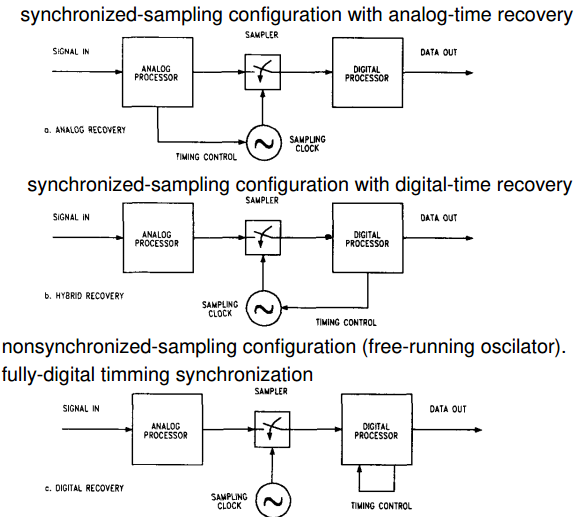
\includegraphics[scale=.3]{figs/tipos_de_sinc_de_relogio.png}
    \end{figure}
    \begin{itemize}
        \item A implementação de um detector completamente digital só é possível com a adoção do método de transmissão assíncrono.
    \end{itemize}
\end{frame}

\begin{frame}[t]
    \frametitle{Método de recuperação de relógio completamente digital}
    \begin{itemize}[<+->]
        \item No caso do método de recuperação de relógio completamente digital, como recuperar o relógio?
        \item \emph{Resposta}: através da \emph{interpolação} do sinal discretizado.
        \item Como a correção do instante de símbolo é implementada?
        \item \emph{Resposta}: utiliza-se três módulos funcionais que integram o chamado sincronizador de relógio \cite{abrantes2010recuperaccao}:
            \begin{itemize}
                \item<.-> Interpolador: responsável por corrigir o instante de amostragem do sinal discreto.
                \item Controlador: utiliza o sinal de erro proveniente do estimador para gerar a parte inteira e fracionária do novo instante de símbolo.
                \item Estimador do atraso de símbolo: gera um sinal de erro em relação à estimativa do atraso de símbolo. É aqui onde a estimação propriamente dita acontece.
            \end{itemize}
    \end{itemize}
\end{frame}

\begin{frame}[t]
	\frametitle{Método de recuperação de relógio completamente digital}
    \begin{itemize}
        \item Dentre os métodos re recuperação de temporização assíncronos (\textit{non-clock-aided}), estes ainda podem ser classificados como segue
    \end{itemize}
    \begin{figure}
        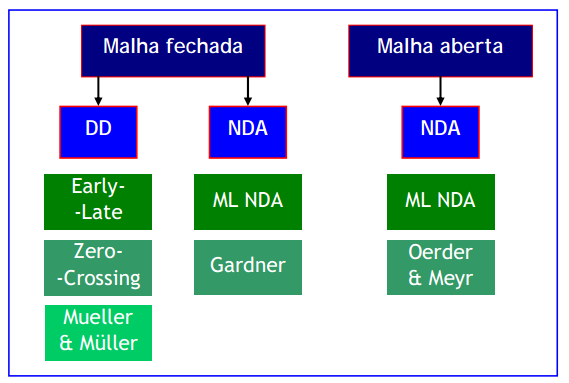
\includegraphics[scale=.45]{figs/tecnicas_estimacao.png}
    \end{figure}
\end{frame}

\begin{frame}[t]
	\frametitle{Método \(M\)-power}
	\begin{itemize}
		\item Como \(h\left( t \right)\) obedece o critério de Nyquist e \(z^*z = \abs{z}^2\) para \(z \in \mathbb{C}\) , a equação \eqref{eq:seg-term1} se torna
		\begin{align}
            \frac{1}{K} \int_{(k-K)T}^{kT} \abs{s(t, \hat{\theta}_{k})}^{2} \diff{t} = \frac{1}{K} \sum_{i = k-K}^{k} \abs{A_i}^2
        \end{align}
        \item Substituindo essas concluções, tem-se
        \begin{align}
            \Lambda(\mathbf{r}_k|\hat{\theta}_{k}) = \textnormal{exp}\left\{ \frac{2}{K} \sum_{i = k-K}^{k} \textnormal{Re} \left\{ x_i A_i^* e^{-j \hat{\theta}_{i}} \right\} - \frac{1}{K} \sum_{i = k-K}^{k} \abs{A_i}^2 \right\}
        \end{align}
	\end{itemize}
	
\end{frame}

\begin{frame}[t]
    \frametitle{Método \(M\)-power}

    \begin{itemize}
        \item A equação anterior se torna mais elegante se observarmos que a métrica de decisão \(\Lambda(\mathbf{r}_k|\hat{\theta}_{k})\) pode ser mutiplicada pelo fator
        \begin{align}
            \textnormal{exp}\left\{ - \frac{1}{K} \sum_{i = k-K}^{k} \abs{x_i}^2 \right\}
        \end{align}
        sem causar consequnências na decisão\footnote{O fator em questão independe de \(\hat{\theta}_{k}\) e, portanto, não altera o valor máximo de \(\Lambda(\mathbf{r}_k|\hat{\theta}_{k})\)}. Sendo assim, tem-se
        \begin{align}
            \Lambda(\mathbf{r}_k|\hat{\theta}_{k}) = \textnormal{exp}\left\{ - \frac{1}{K} \sum_{i = k-K}^{k} \abs{x_i e^{-j \hat{\theta}_i} - A_i}^2 \right\}
        \end{align}
    \end{itemize}

\end{frame}

\begin{frame}[t]
	\frametitle{Método \(M\)-power}
	\begin{itemize}
		\item Para o sinal M-PSK, tem-se que \(A_k = e^{j\frac{2\pi m}{M}}\), em que \(m \in \left\{ 0, 1, \dots, M-1 \right\}\). Recordando que \(\abs{z_1 \pm z_2}^2 = \abs{z_1}^2 \pm 2 \textnormal{Re}\left\{ z_1 z_2^* \right\} + \abs{z_2}^2\), para \(z_1, z_2 \in \mathbb{C}\), e ignorando os termos que não interferem na métrica, o função log-verossimilhança pode ser escrita como
		\begin{align}
            \Lambda_L(\mathbf{r}_k|\hat{\theta}_{k}) = \ln{\Lambda(\mathbf{r}_k|\hat{\theta}_{k})} = \sum_{i = k-K}^{k} \textnormal{Re}\left\{ x_i e^{-j \left(\frac{2\pi m}{M}+\hat{\theta}_i\right)} \right\} % TODO: a parte A_k no mengali ficou o cunjulgado do que está aqui, verificar
        \end{align}
	\end{itemize}
	
\end{frame}

\begin{frame}[t]
	\frametitle{Método \(M\)-power}
	\begin{itemize}
        \item Mas recorde que \(2\textnormal{Re}\left\{ z \right\} = z + z^*\) e
        \begin{align}
            \left( z_1 + z_2 \right)^p = \sum_{q=0}^{p} \begin{pmatrix}
                p \\
                q
            \end{pmatrix} z^p z^{q-p}
        \end{align}
        \item Realizando essas substituições e expandindo a exponencial complexa, tem-se
        \begin{align}
            \Lambda_L(\mathbf{r}_k|\hat{\theta}_{k}) = \sum_{i=k-K}^{k} \sum_{p=0}^{\infty}\frac{1}{p!} \sum_{q=0}^{p} \begin{pmatrix}
                p \\
                q
            \end{pmatrix}
            x^{q}_{i} \left( x^{*}_{i} \right)^{p-q} e^{j\left( p-2q \right)\hat{\theta}_i} e^{j\frac{2\pi m}{M}}
        \end{align}
        
    \end{itemize}
\end{frame}

\begin{frame}[t]
	\frametitle{Método \(M\)-power}
	\begin{itemize}
		
		\item Para uma SNR suficientemente baixa, a seguinte aproximação é válida \cite{mengali2013synchronization}:
        \begin{align}
            \Lambda_L(\mathbf{r}_k|\hat{\theta}_{k}) \approx \textnormal{Re}\left\{e^{-jM \hat{\theta}_k} \sum_{i=k-K}^{k} x_{k}^{M} \right\}
        \end{align}
        \item O valor que \(\hat{\theta}_{k}\) que maximiza a função log-verossimilhança é dada por
        \begin{align}
            \hat{\theta}_{k} = \frac{1}{M} \textnormal{Arg}\left\{ \sum_{i=k-K+1}^{k} x_{i}^M \right\}
        \end{align}
	\end{itemize}
\end{frame}

\section{Implementação}
\begin{frame}[c]
    \frametitle{Implementação}

    \begin{figure}
        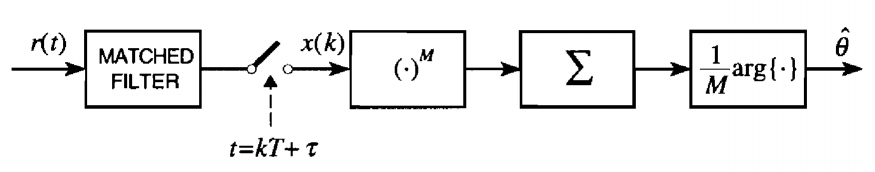
\includegraphics[scale=.3]{figs/m-power.png}
    \end{figure}
\end{frame}

\section{Próxima aula}
\begin{frame}[t]
    \frametitle{Implementação}

    \begin{itemize}
        \item Apesentação de algumas arquiteturas de estimadores de tempo de símbolo.
    \end{itemize}
\end{frame}